\documentclass[12pt]{article}
\usepackage[a4paper, top=16mm, text={170mm, 248mm}, includehead, includefoot, hmarginratio=1:1, heightrounded]{geometry}
\usepackage{amsmath,amssymb,mathrsfs,amsthm,tikz,shuffle}
\usepackage{dsfont}


\theoremstyle{definition}
	\newtheorem{para}{}[section]
		\renewcommand{\thepara}{\thesection.\arabic{para}}
	\newtheorem{exa}[para]{Example}
\theoremstyle{plain}
	\newtheorem{lem}[para]{Lemma}
	\newtheorem{thm}[para]{Theorem}
	\newtheorem{pro}[para]{Proposition}
\renewcommand{\proofname}{Proof}


%+++++++++++++++++++++++数学字体的设置++++++++++++++++++++++++++++++++++++++++%
\newcommand{\me}{\mathrm{e}}  % for math e
\newcommand{\mi}{\mathrm{i}} % for math i
\newcommand{\dif}{\mathrm{d}} %for differential operator d
\newcommand{\cvec}[1]{\!\vec{\,#1}}
\newcommand{\Ptimes}{\,\overset{\otimes }{,}\,}
\DeclareSymbolFont{lettersA}{U}{txmia}{m}{it}
 \DeclareMathSymbol{\piup}{\mathord}{lettersA}{25}
 \DeclareMathSymbol{\muup}{\mathord}{lettersA}{22}
 \DeclareMathSymbol{\deltaup}{\mathord}{lettersA}{14}
 \newcommand{\uppi}{\piup}

\pagestyle{plain}

\begin{document}

\section{Intro}

\section{Map}

In this section we present a proof to the statement:
\begin{thm}
For an arbitrary product of M polynomials $P=\prod_{j=1}^M p_j^{\alpha_j}$, $p_j=\sum_{I_j} a_{I_j} x^{I_j}$ with $a_{I_j}\geq 0$ for all $I_j$ and
 \[
	x^{I_j}=\prod_{i=1}^N x_i^{n^{I_j}_i},
\]
whose Newton polytope is defined as the Minkowski sum  $N_P=\sum_j \alpha_j N(p_j)$, each $N(p_j)$ being the convex hull of vectors $\{\mathbf{n}^{I_j}=(n^{I_j}_1,\dots,n^{I_j}_N)\}$. Then the scattering map:
\[
	\mathbf X(x)=\frac{\partial \log P}{\partial \log \mathbf x},
\]
where $x_i\in (0,\infty)$ for all $i$, is an one-to-one map between $(0,\infty)^N$ and the interior of $N_P$. 

\end{thm}

The proof is finished in two steps.:
\paragraph{Step 1: M=1}
Consider a unique polynomial $p=\sum_{I} a_I x^I$ with $a_I\geq 0$ for all $I$. The scattering map now reads:
\[
	\mathbf X(x)=\frac{\partial \log p}{\partial \log \mathbf x},
\]
where $x_i\in (0,\infty)$ for all $i$.

Firstly, without loss of generality, we can assume that the matrix $(n_i^I)$ has full rank. Therefore $\dim (N(p))=N$. If not, there exists $\mathbf s\neq 0$ such that $\mathbf s \cdot \mathbf n^I=0$ for all $I$. In this case,
\[
	\mathbf s\cdot\mathbf X=\mathbf s\cdot\frac{\partial \log p}{\partial \log \mathbf x}=0.
\]
Therefore, one can project $\operatorname{im}(\mathbf X)$ by setting some $x_i=1$ so that there's no more vector $\mathbf s$ such that $\mathbf s\cdot \mathbf n^I=0$ for all $I$. Conversely, one can recover the original image by solving these equations $\mathbf s\cdot\mathbf X=0$. 

Next we show that interior points of $N(p)$ are in the $\operatorname{im}(\mathbf{X})$.
Let $\mathbf{\Lambda}$ be a interior point in $N(p)$ defined by 
\[
	\mathbf \Lambda=\sum_{I}\lambda_I\mathbf n^I
	=\frac{\partial}{\partial \log \mathbf x}\sum_{I}\lambda_I \log x^I
\]
where $\sum_I \lambda_I=1$ and $\lambda_I > 0$. Equations $\mathbf X(x)=\mathbf \Lambda$ are 
\[
\begin{aligned}
	0=\frac{\partial }{\partial \log \mathbf x}\left(
	\log p-\sum_{I}\lambda_I \log x^I
	\right)=\frac{\partial }{\partial \log \mathbf x}\left(
	\log F(\mathbf x)
	\right)=\frac{1}{F(\mathbf x)}\frac{\partial F(\mathbf x)}{\partial \log \mathbf x}
\end{aligned}
\]
where
\[
	F(\mathbf x)=\sum_I a_I x^I\prod_J (x^{-J})^{\lambda_J}.
\]
Let $\mathbf y=\log \mathbf x$, and then
\[
	\begin{aligned}
		F(\mathbf y)
		&=\sum_I a_I \exp\left(\mathbf{y}\cdot \left(\mathbf{n}^I-\mathbf{\Lambda}\right)\right)
	\end{aligned}
\]
so we only need to show that $F(\mathbf y)$ has saddle points in $\mathbb R^N$ because $F>0$ for all $\mathbf y$. To see it, we firstly notice that $F(\mathbf y)$ is a strict convex function of $\mathbf y$. In fact, the Hessian of $F(\mathbf y)$ is 
\[
	H_{ij}(\mathbf y)=\frac{\partial^2}{\partial y_i\partial y_j}F(\mathbf y)=\sum_I a_I \exp\left(\mathbf{y}\cdot \left(\mathbf{n}^I-\mathbf{\Lambda}\right)\right)\left(\mathbf{n}^I-\mathbf{\Lambda}\right)_i\left(\mathbf{n}^I-\mathbf{\Lambda}\right)_j.
\]
For any $\mathbf v\neq 0$, 
\[
	\sum_{i,j}v_iv_jH_{ij}=\sum_I a_I \exp\left(\mathbf{y}\cdot \left(\mathbf{n}^I-\mathbf{\Lambda}\right)\right) \left(\mathbf v\cdot (\mathbf{n}^I-\mathbf{\Lambda})\right)^2 >0.
\]
It cannot vanish because that it only happens when $\mathbf v\cdot (\mathbf{n}^I-\mathbf{\Lambda})=0$ for all $I$, but we have assumed $\{\mathbf n^I\}$ has full rank.

For a strict convex function $F(\mathbf y)$ on $\mathbb R^N$, it has a unique minimal in $\mathbb R^N$ iff it does not take its minimal when $\mathbf{y}$ goes to infinity along any direction. In our case, we only need that for any $\mathbf{y}\neq 0$ and $\mathbf\Lambda \in (N(p))^\circ $, there exist some $I$ such that  
\[
	\mathbf{y}\cdot (\mathbf{n}^I-\mathbf{\Lambda})>0
\]
and if $\mathbf\Lambda \not\in N(p)$, there exist some $\mathbf{y}\neq 0$ such that the exponentials are all negative, then $F(t\mathbf y)\to 0$ when $t\to \infty$, which is direct result of convexity of $N(p)$.

\begin{figure}[htbp]
\centering
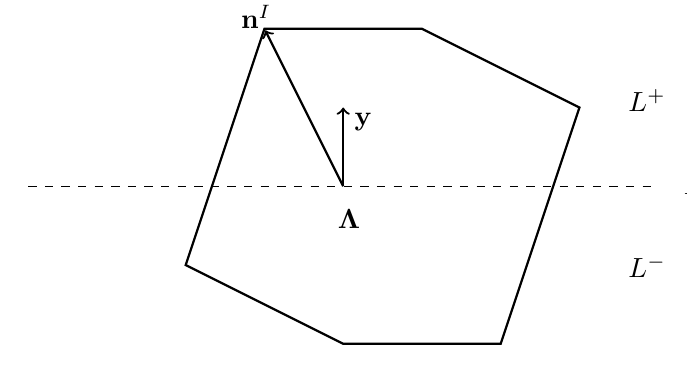
\begin{tikzpicture}
\draw[black,thick](3,0)--(1,0)--(0,-3)--(2,-4)--(4,-4)--(5,-1)--cycle;
\draw[black,dashed](-2,-2)--(6,-2);
\draw[->,black,thick](2,-2)--(2,-1);
\draw[->,black,thick](2,-2)--(1.01,-0.02);
\put(55,-72){$\mathbf{\Lambda}$};
\put(61,-35){$\mathbf{y}$};
\put(180,-60){$L$};
\put(160,-30){$L^+$};
\put(160,-90){$L^-$};
\put(20,0){$\mathbf{n}^I$};
\end{tikzpicture}

\caption{}
In fact, if $\mathbf\Lambda \in (N(p))^\circ$, for a given $\mathbf y\neq 0$, the hyperplain $L$ with normal vector $\mathbf y$ crossing $\mathbf \Lambda$ divides the space $\mathbb R^N$ into semi-spaces $L^+$ and $L^-$, then $\mathbf{n}^I$ in $L^+$ are what we are looking for. Conversely, if $\mathbf\Lambda \not\in N(p)$, one can find a hyperplain $L$ such that $N(p)\subset L^-$, then the normal vector of $L$ gives the wanted direction. 

\end{figure}






Therefore, we have proven that $F(\mathbf y)$ has a unique minimal in $\mathbb R^N$ when $\mathbf \Lambda \in (N(p))^\circ$ and no minimal in $\mathbb R^N$ when $\mathbf \Lambda \not\in N(p)$. Hence, 
\[
	\mathbf X(x)=\frac{\partial \log p}{\partial \log \mathbf x},
\]
is an one-to-one map between $(0,\infty)^N$ and the interior of $N(p)$, which finishes the first step.



\paragraph{Step 2: general M}
Generally, let $\mathbf{\Lambda}$ be a interior point in Minkowski sum $\sum_p \alpha_p N(p)$ corresponding to $P=\prod_p p^{\alpha_p}$ defined by 
\[
	\mathbf{\Lambda}
	=\sum_p \alpha_p \mathbf{\Lambda}_p
	=\sum_p \alpha_p \sum_{I_p}\lambda_{I_p}\mathbf{n}^{I_p}
	=\frac{\partial}{\partial \log \mathbf{x}}\sum_{p}\alpha_p\sum_{I_p}\lambda_{I_p} \log x^{I_p}
\]
where $\sum_{I_p} \lambda_{I_p}=1$ and $\lambda_{I_p} > 0$. Equations $\mathbf{X}(x)=\mathbf{\Lambda}$ are 
\[
\begin{aligned}
	0=\frac{\partial }{\partial \log \mathbf{x}}\left(
	\log P-\sum_{p}\alpha_p\sum_{I_p}\lambda_{I_p} \log x^{I_p}
	\right)&=\frac{\partial }{\partial \log \mathbf{x}}\left(
	\log \left(\prod_p F_p^{\alpha_p}\right)
	\right),
\end{aligned}
\]
where
\[
	\begin{aligned}
		F_p(\mathbf y)&=\sum_{I_p} a_{I_p} \exp\left(\mathbf{y}\cdot \left(\mathbf{n}^{I_p}-\mathbf{\Lambda}_p\right)\right).
	\end{aligned}
\]
Write
\[
	F(\mathbf y)=\prod_p F_p(y)^{\alpha_p},
\]
we only need to show that $F(y)$ has a unique saddle point in $\mathbb R^N$.

We assume that $\alpha_p>0$ for all $p$. Here, $F(\mathbf y)$ is no longer a strict convex function. However, take a positive number $\alpha_0$ such that $\alpha_0< \alpha_p$ for all $p$, consider a new function
\[
	F(y)^{1/\alpha_0}=\prod_p F_p(y)^{\alpha_p/\alpha_0},
\]
since $F_p$ are convex functions and $\alpha_p/\alpha_0>1$, $F_p(y)^{\alpha_p/\alpha_0}$ are convex functions, so is their product. Since $F(y)^{1/\alpha_0}$ has the same minimums as $F(y)$, so we can further assume that $\alpha_p>1$ for all $p$.

Finally, we claim that $F(y)$ does not take minimum when $\mathbf{y}$ goes to infinity along any direction. It is because that for a given $\mathbf{y}$ and each $p$, $F_p(t\mathbf{y})\to \infty$ when $t\to \infty$, so does $F(t\mathbf{y})=\prod_p F_p(t\mathbf{y})^{\alpha_p}$. Therefore, equation $\mathbf{X}(x)=\mathbf{\Lambda}$ has a unique solution.

\section{Blow up}

Consider the following integral
\[
	\int_{\mathbb R_+^d}\frac{d x_1}{x_1} \cdots \frac{d x_d}{x_d} x_1^{n_1}\cdots x_d^{\alpha' n_d} P(x_1,\dots,x_d)^{-\alpha' c}, 
\]
where $P$ is a polynomial, here we can further assume that $P(0,\dots,0)\neq 0$. When $\alpha'\to 0$, the integral diverge, we want to calculate the leading term of $(\alpha')^{-1}$ of this integral. blabla

Let's first consider the one-dimensional example, the Beta function 
\[
	B(\alpha' a,\alpha' b)=\int_0^1 \frac{dt}{t(1-t)} t^{\alpha' a}(1-t)^{\alpha' b}=\int_{\mathbb R_+}\frac{dt}{t}t^{\alpha' a}(1+t)^{\alpha'(a+b)}.
\]
To calculate the integral, we can decompose the integral by 
\[
	\biggl(\int_{0}^\epsilon +\int_\epsilon^{1/\epsilon}+\int_{1/\epsilon}^\infty\biggr)\frac{dt}{t} t^{\alpha' a}(1+t)^{\alpha'(a+b)}.
	\]
The middle integral is finte when $\alpha'\to 0$ so that do not contribute the leading term, the first integral is 
	\[
		\int_0^\epsilon \frac{dt}t t^{\alpha' a}(1+t)^{\alpha'(a+b)}
	\sim \int_0^\epsilon \frac{dt}t t^{\alpha' a} 
	= \frac{\epsilon^{\alpha' a}}{\alpha'a} \sim \frac{1}{\alpha'a},
\]
and the last integral is 
\[
	\int_{1/\epsilon}^\infty \frac{dt}t t^{\alpha' a}(1+t)^{\alpha'(a+b)} 
	= \int_0^\epsilon \frac{dt}{t} t^{\alpha' b}(1+t)^{\alpha' (a+b)}
	\sim \frac{1}{\alpha' b},
\]
so the leading term of this integral is 
\[
	B(\alpha' a,\alpha' b)\sim\frac 1{\alpha'}\biggl(\frac1a+\frac1b\biggr).
\]

There's one important lesson from the above simple integral, the leading terms of the integral comes from the vertices of the regions. 


\section{General prescription of pole subtraction}

\end{document}